% EBP course: session 7
% Thomas Klee
% 2019-03-13

% Preamble
\documentclass{beamer}
\usetheme{Singapore}
\usefonttheme[onlysmall]{structurebold}
\setbeamerfont{title}{shape=\itshape,family=\rmfamily}
\usepackage{graphicx}
\usepackage[english]{babel}
\usepackage[utf8x]{inputenc}
\usepackage{amsfonts, amsmath, amsthm, amssymb} % for math fonts, symbols and environments
\usepackage{xcolor}
\usepackage{booktabs}
\usepackage{ctable} % for command-driven tables
\usepackage{wasysym} 
\hypersetup{colorlinks, allcolors = ., urlcolor = blue,} % to change color of URL from black to blue
\usepackage[natbibapa]{apacite}
\beamertemplatenavigationsymbolsempty % uncomment to add slide navigation symbols to each slide
\usepackage{appendixnumberbeamer}  % to suppress page numbers on extra slides
\setbeamertemplate{footline}[frame number] % to add slide numbers

% activate following line for custom appearance
% \usepackage{beamerthemesplit} 

\mode<presentation>

% information for title slide
\title{Single-Subject Data, Part 2}
\subtitle{}
\author{Evidence-Based Practice in Speech-Language Therapy \\ (SHSC 2033)}
\institute{Session 7}
\date{Thomas Klee \& Elizabeth Barrett}
\titlegraphic{
\includegraphics[width=6cm]{images/logo_CE_C.jpg}} % HKU logo

\begin{document}

% create title slide with information above
\begin{frame}
	\titlepage
\end{frame}

% 
\begin{frame}{Outline}
	\begin{enumerate}
	\item Types of designs
		\begin{itemize}
		\item Withdrawal (reversal) designs 
		\item Multiple baseline designs
		\item Alternating-treatments designs
		\item Other designs
		\end{itemize}
	\item Data analysis, reporting standards, critical appraisal 
	\item Group discussion
	\end {enumerate}
\end{frame}

\section{Introduction}

% 
\begin{frame}{Key features of SSDs}
	\begin{itemize}
	\item Good SSDs are \alert{logical} in design. They should be designed so that alternative explanations for the results are minimised beforehand. This means trying to reduce \textbf{sources of bias} as far as possible.
	\item They are \alert{flexible} intervention designs. The basic designs can be adapted to different clinical situations.
	\end{itemize}
\end{frame}

% 
\begin{frame}{Judging intervention effectiveness}
Two questions to ask:
	\begin{enumerate}
	\item Was there a change?
	\item Was the change due to intervention?
	\end{enumerate}
\end{frame}

\section{Types of Designs}

\begin{frame}
\begin{center}
\Huge{Withdrawal Designs}
\end{center}
\end{frame}

% 
\begin{frame}{Withdrawal designs\footnote{\tiny{\citet{Kearns1986}}}}
	\begin{itemize}
	\item A-B-A design (at a minimum)
	\item Allows a treatment--no treatment comparison
	\item Clinical research question: \\
		 \emph{``Does \alert{treatment}, with all of its components, result in improved performance relative to \alert{no treatment?"}}
	\item Can be used if it's logical to expect that the intervention effect is likely to reverse if it's withdrawn
	\end{itemize}
\end{frame}

% 
\begin{frame}{Example}	
	\begin{itemize}
	\item Is \emph{X} effective in treating hypertension (high blood pressure)?
		\begin{itemize}
		\item[-] \emph{X} could be exercise, diet, meditation, medication, etc.
		\end{itemize}
	\item What evidence exists at a group level?
		\begin{itemize}
		\item[-] Is there a recent SR of RCTs available? 
		\item[-] If not, has an RCT been done?
		\item[-] If not, have other kinds of studies been done?
		\end{itemize}
	\item Example clinical question: \\ 
		\emph{``Does X lower \alert{this patient's} blood pressure?"}  
	\end{itemize}
\end{frame}

% 
\begin{frame}{AB design}	
	\begin{center}
	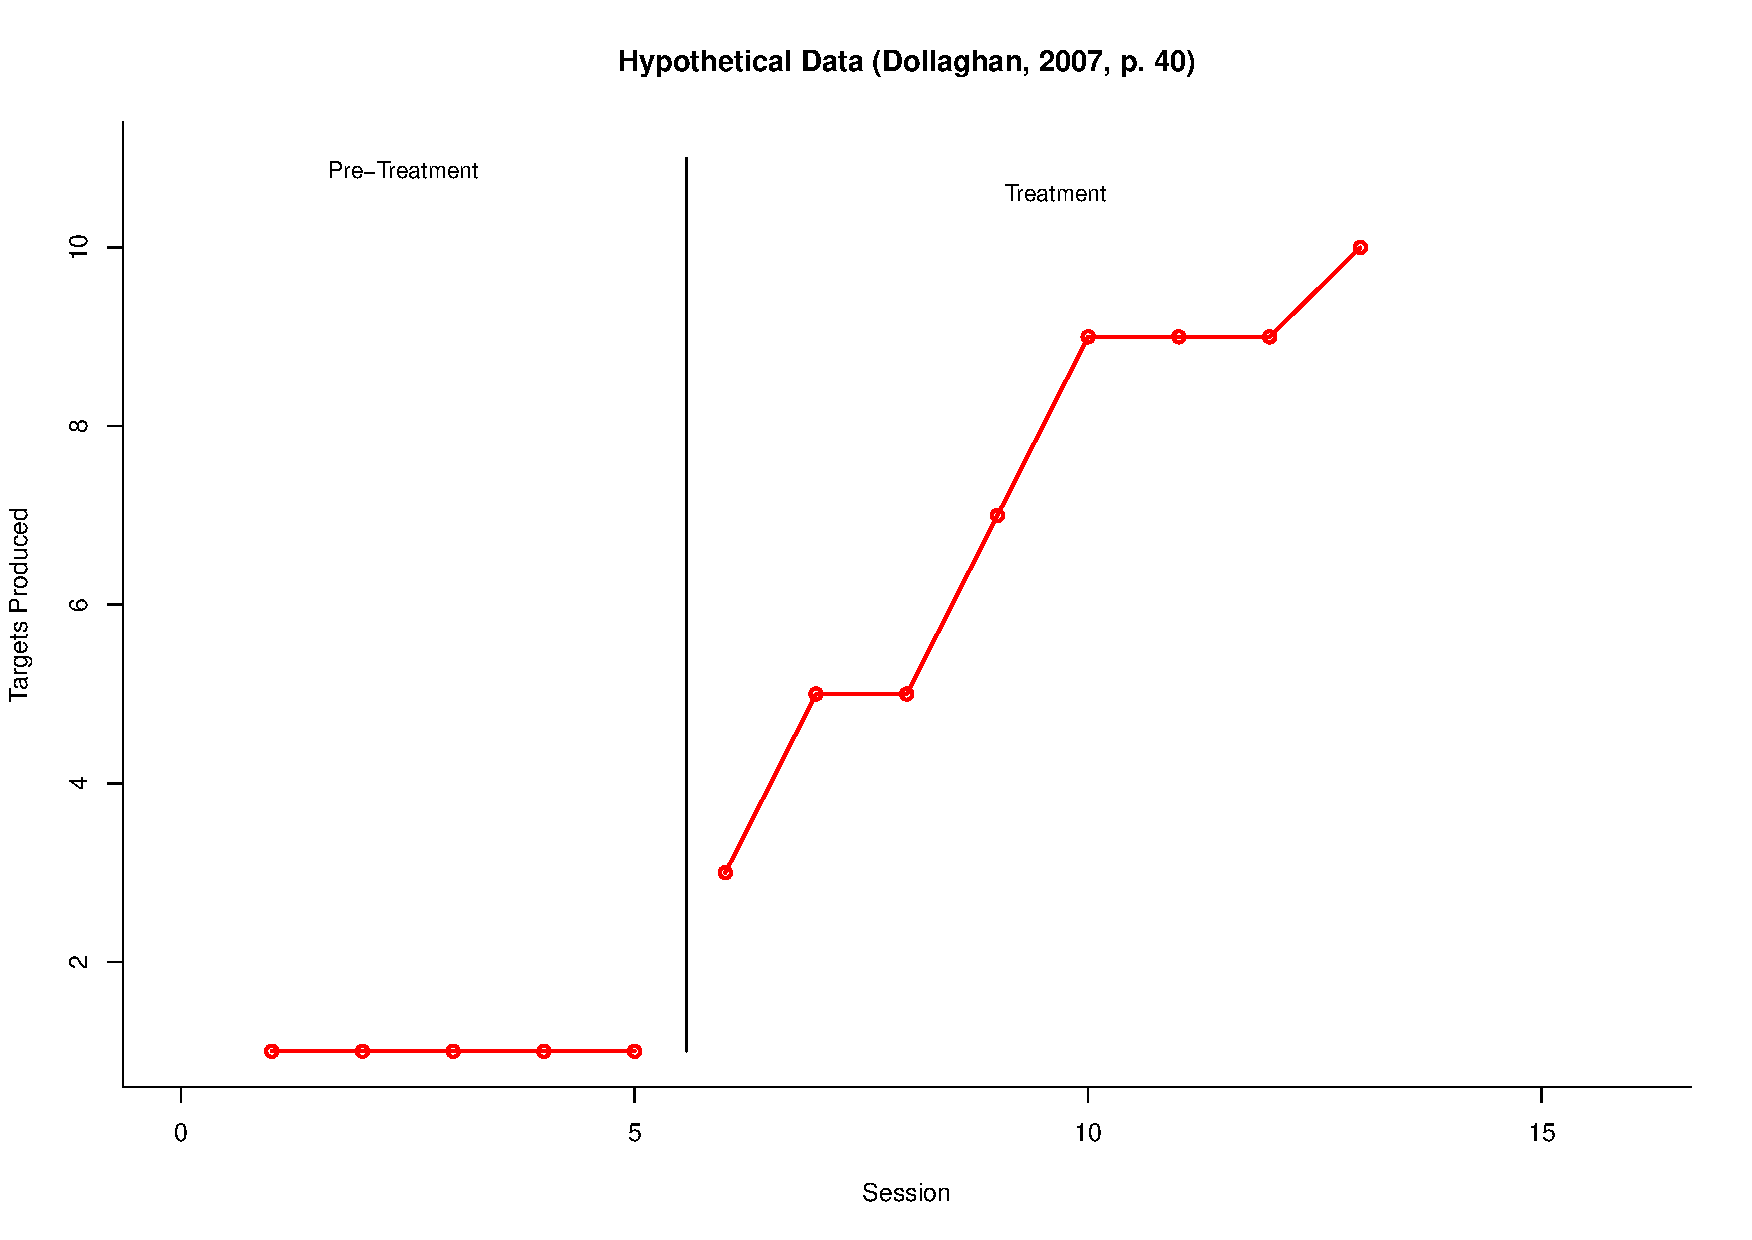
\includegraphics[width=10cm]{SSD/ABplot.pdf}
	\end{center}
\end{frame}

% 
\begin{frame}{AB design with replication\footnote{\tiny{Although graph is from \citet[p. 169]{Horner2005}, it might also illustrate lowered blood pressure as a result of intervention, if the y-axis were changed to systolic blood pressure, for instance.}}}
%	\begin{center}
	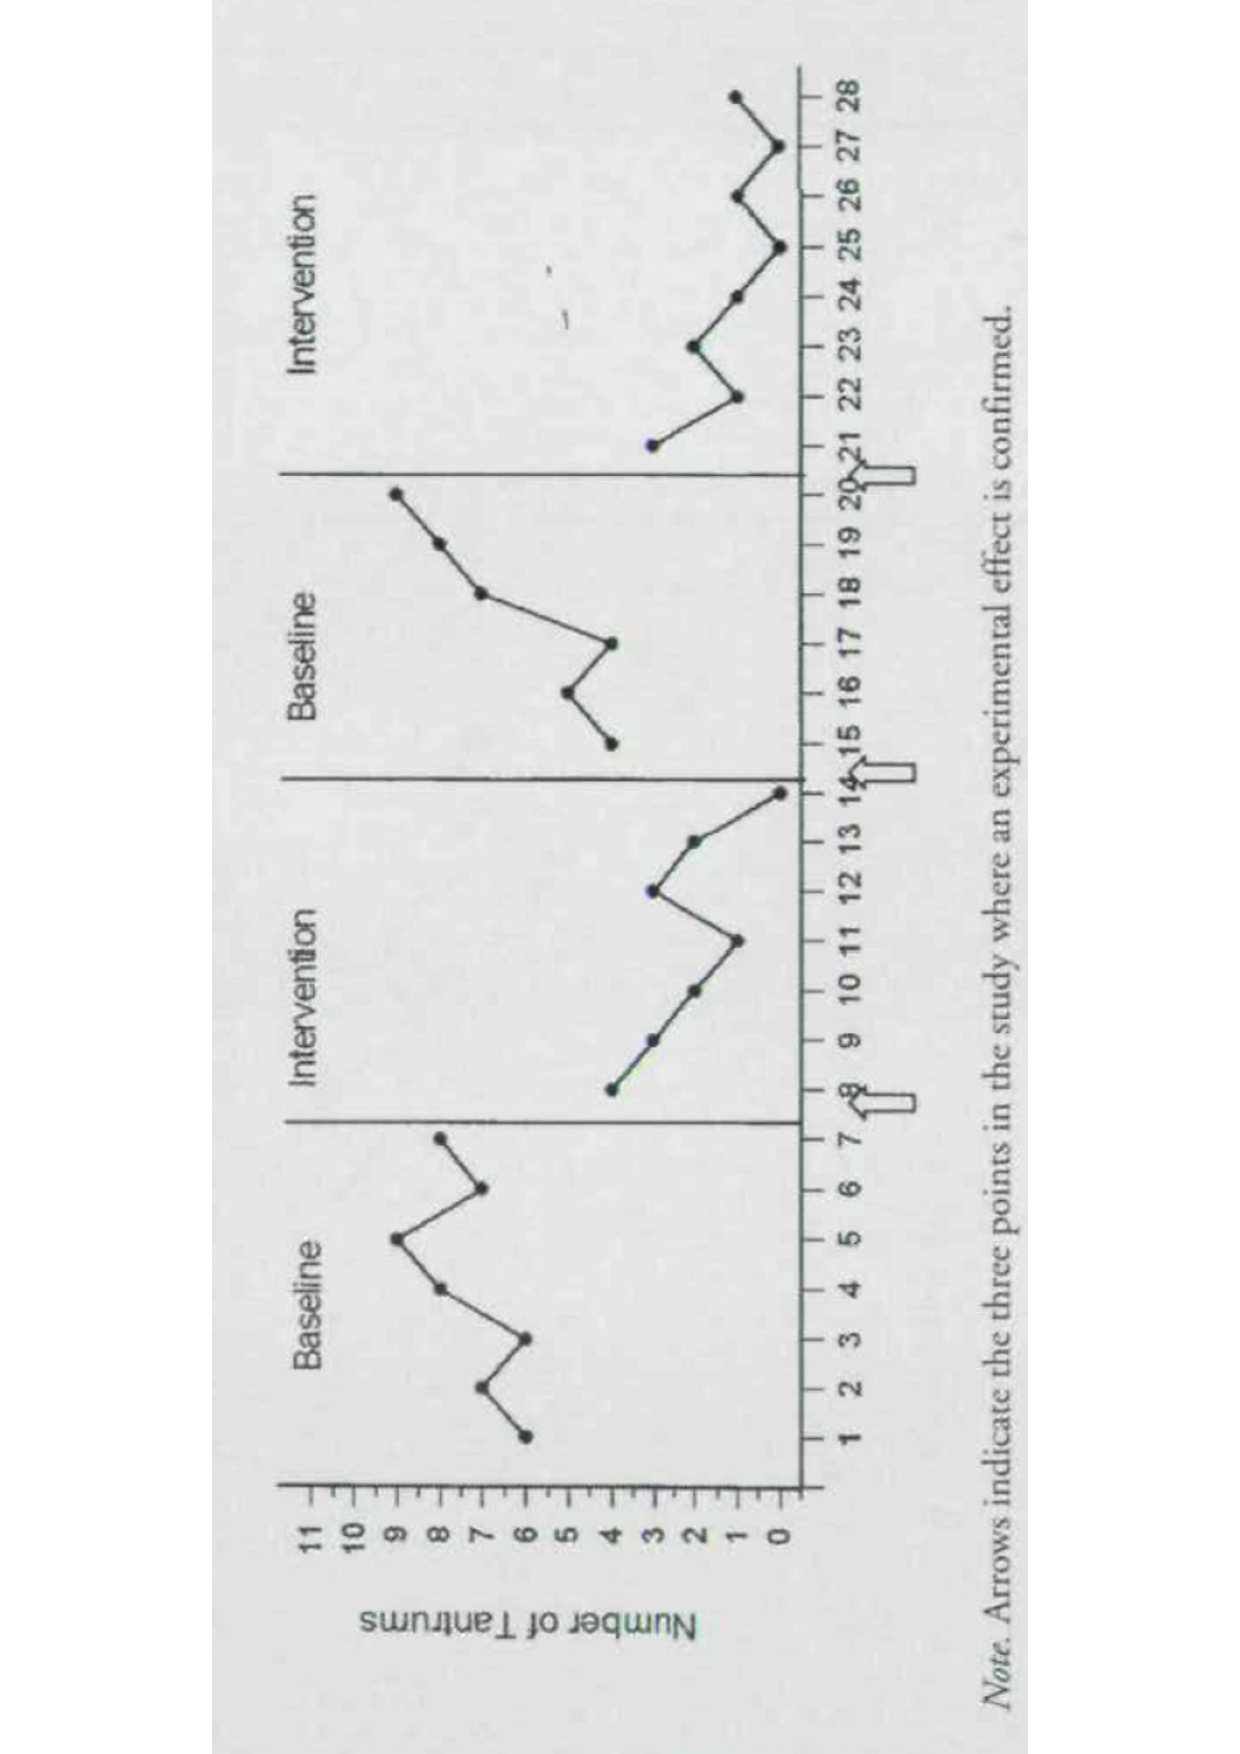
\includegraphics[angle=270, width=10cm]{images/horner2005_p169.pdf}
%	\end{center}
\end{frame}

\begin{frame}
\begin{center}
\Huge{Multiple Baseline Designs}
\end{center}
\end{frame}

% 
\begin{frame}{Multiple baseline designs\footnote{\tiny{\citet{Kearns1986}}}}
	\begin{itemize}
	\item Allows a treatment--no treatment comparison
	\item Clinical research question: \\
		 \emph{``Does \alert{treatment}, with all of its components, result in improved performance relative to \alert{no treatment?"}}
	\item Can be used if functionally independent behaviours or settings are available, or if similar clients are available.
	\item Types of multiple baseline designs
		\begin{itemize}
		\item[-] across behaviours
		\item[-] across settings
		\item[-] across subjects
		\end{itemize}
	\end{itemize}
\end{frame}

% 
\begin{frame}{Example\footnote{\tiny{\citet[Fig. 1]{Rudolph2014}}}}
	\begin{center}
	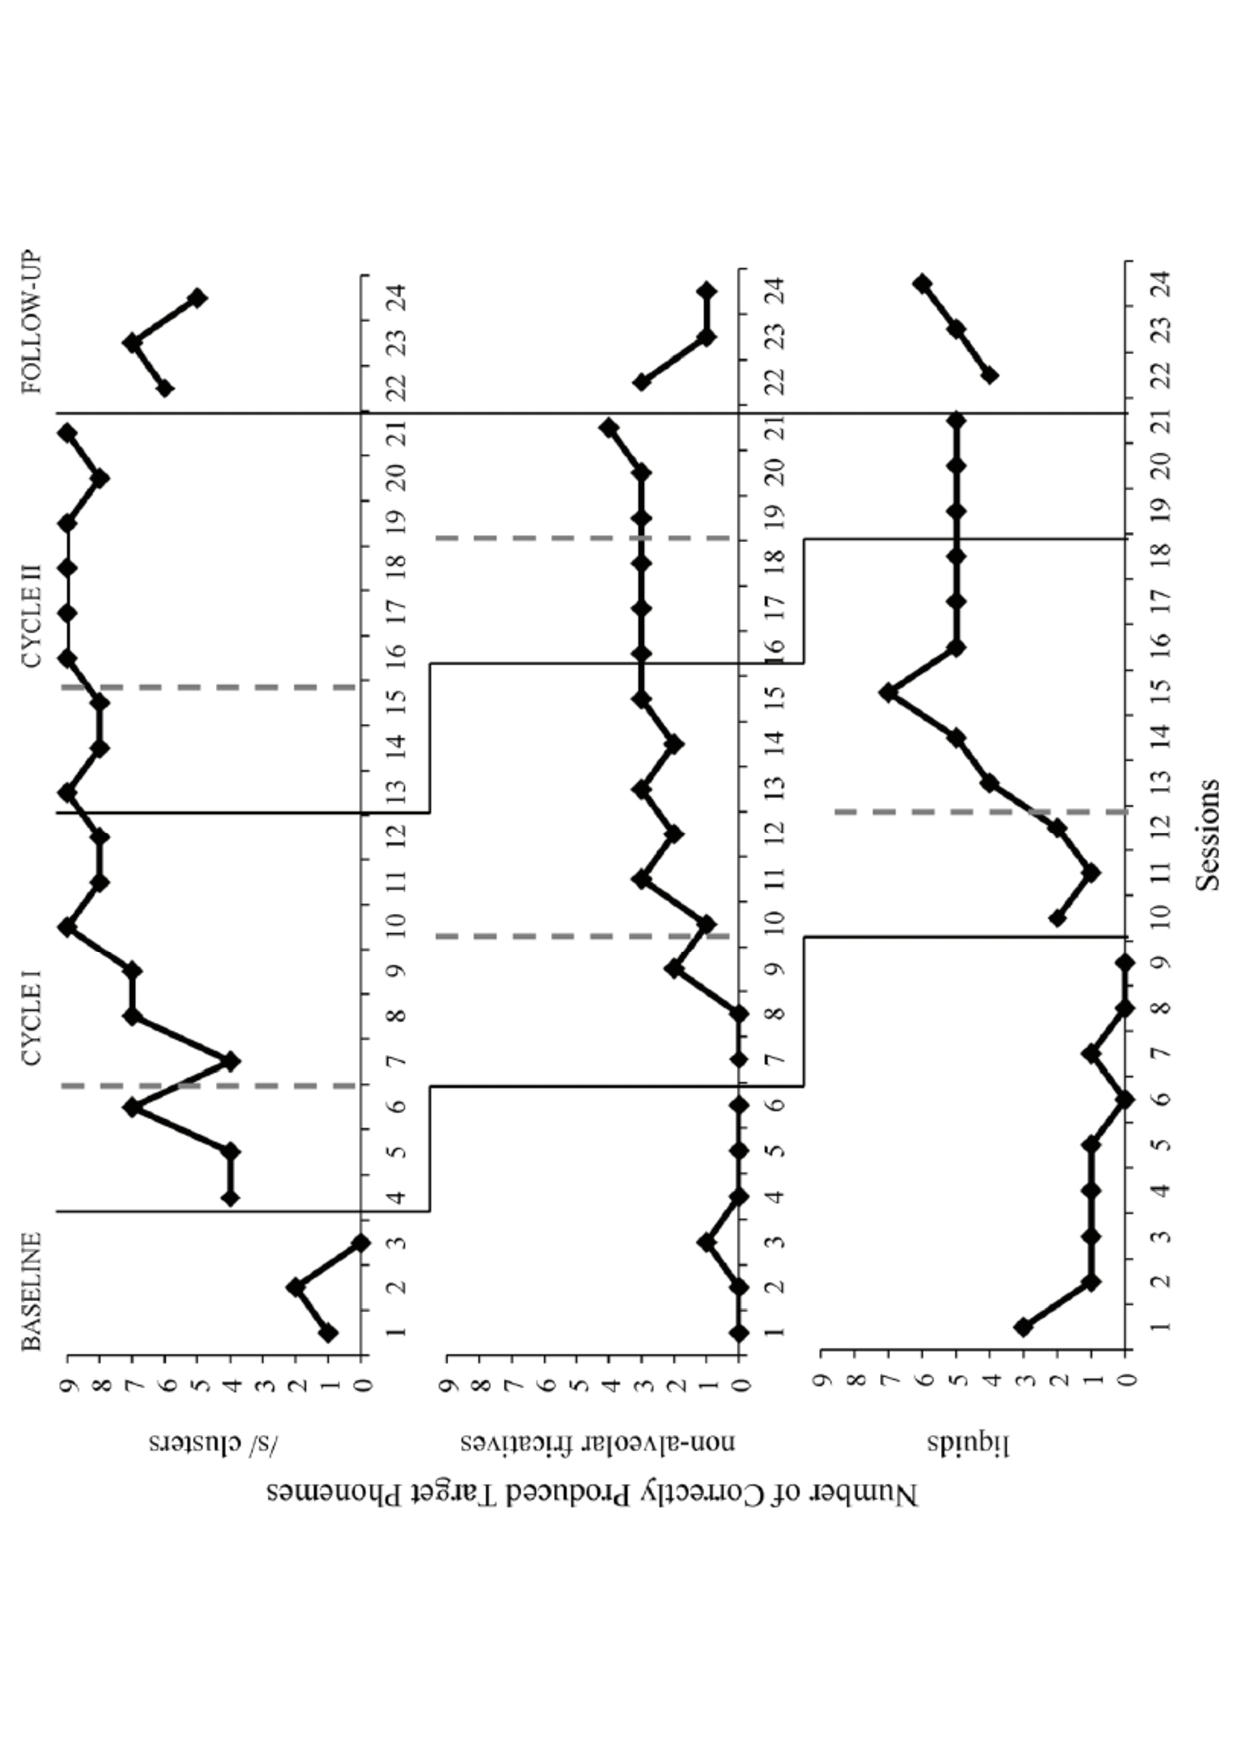
\includegraphics[angle=270, width=9cm]{images/rudolph_wendt_Fig1.pdf}
	\end{center}
\end{frame}

\begin{frame}
\begin{center}
\Huge{Alternating Treatments Designs}
\end{center}
\end{frame}

% 
\begin{frame}{Alternating treatments designs\footnote{\tiny{\citet[p. 211]{Kearns1986}}}}
	\begin{itemize}
	\item Useful for comparing different intervention approaches
	\item Treatments to be compared are administered in a rapid, alternating manner.
	\item Confounding factors that may influence treatment effectiveness are counterbalanced.
		\begin{itemize}
		\item[-] Examples: clinicians, order of treatment presentation
		\end{itemize}
	\item This design does not require a baseline measure, but including one makes it possible to compare treatment conditions with no treatment.
	\item ATDs are procedurally complex to conduct.
	\end{itemize}
\end{frame}

% 
\begin{frame}{Example\footnote{\tiny{\citet{Olswang1983}}}}
	\begin{itemize}
	\item Treatment efficacy study of 4 children with developmental language disorder
	\item Study aim: to compare \alert{object manipulation} and \alert{picture identification} for facilitating single-word production 
	\item Alternating treatment design 
	\item Ages of children: 23--40 months
	\item Expressive vocabulary size: 6--50 words
	\end{itemize}
\end{frame}

% 
\begin{frame}{Alternating treatment design\footnote{\tiny{Olwang et al. (1983) results redrawn by \citet[p. 211]{Kearns1986}}}}
	\begin{center}
	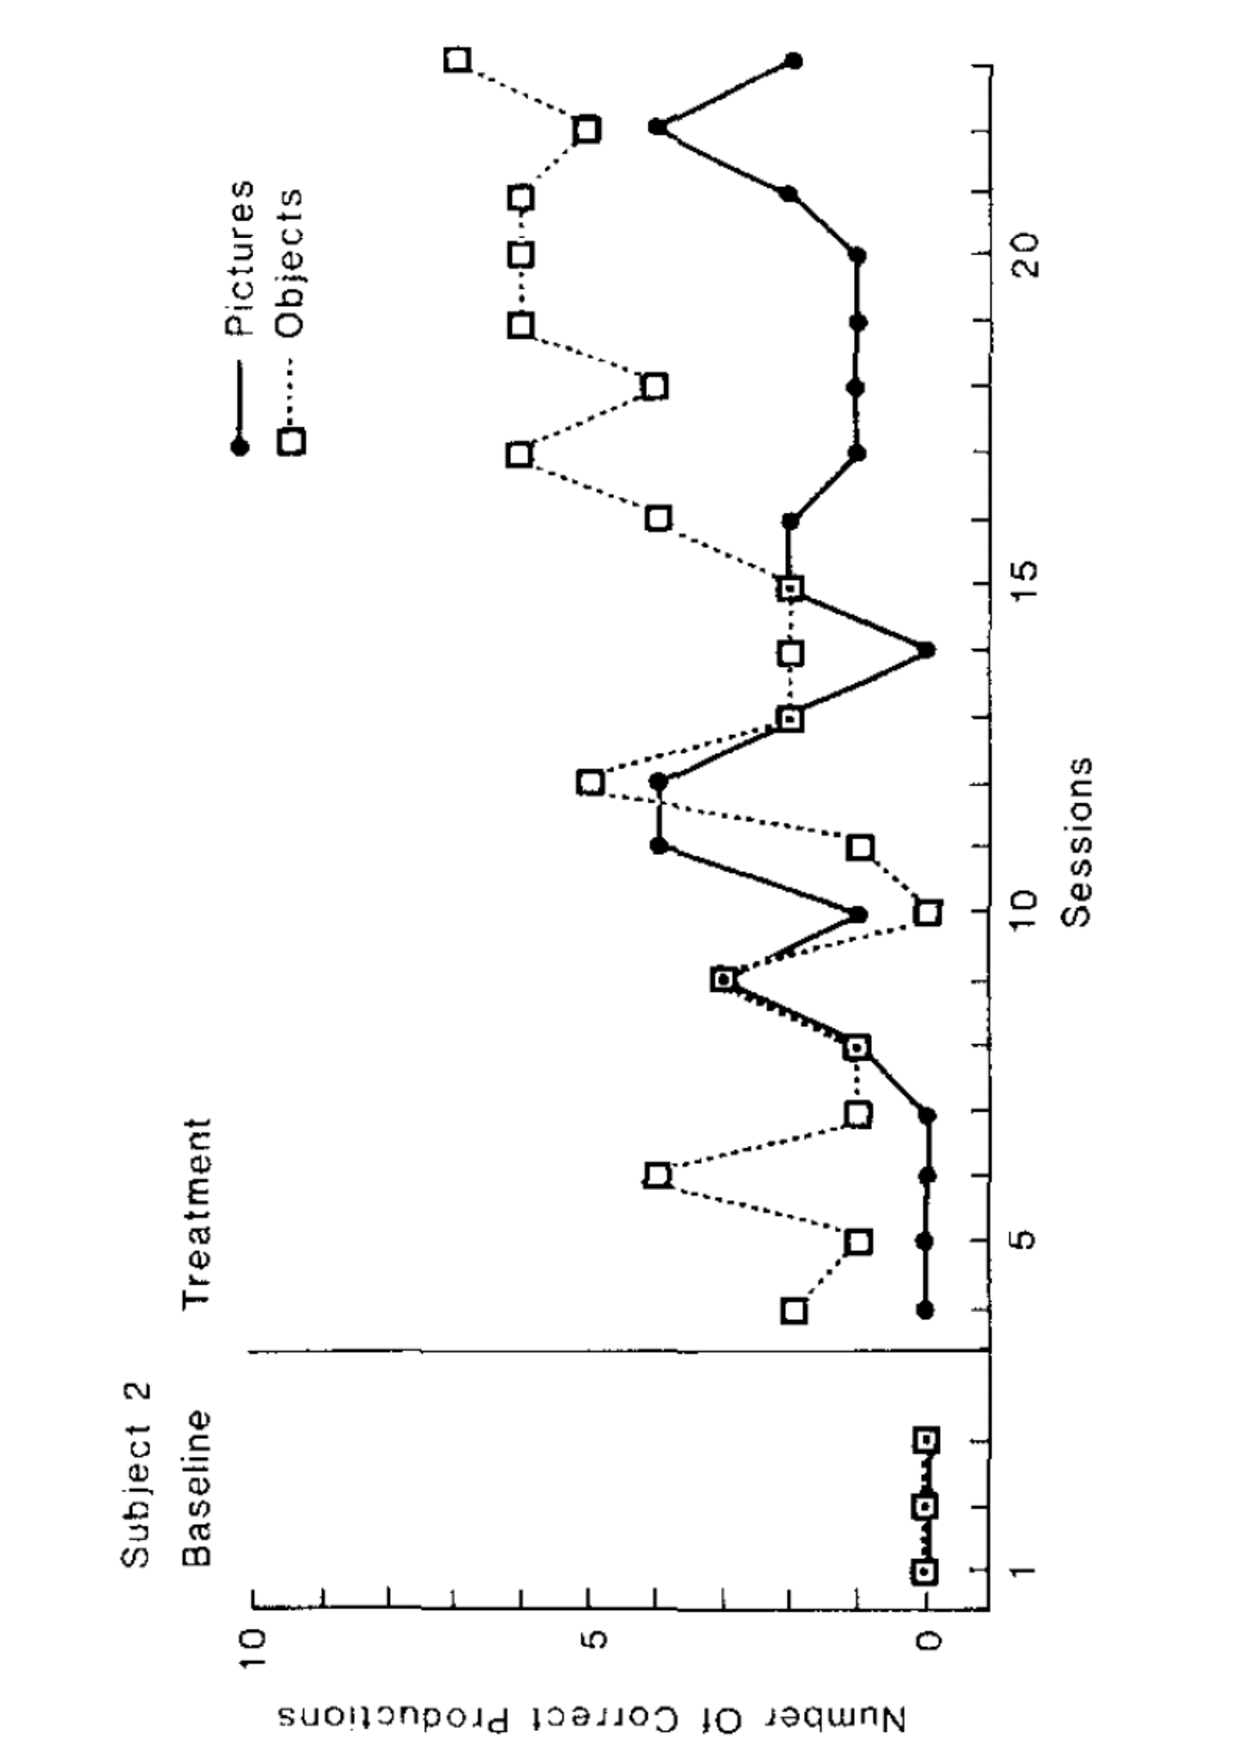
\includegraphics[angle=270, width=9cm]{images/kearns1986_p211.pdf}
	\end{center}
\end{frame}

% 
\begin{frame}{Interaction design\footnote{\tiny{\citet[Fig. 3]{Kearns1986}}}}
	\begin{center}
	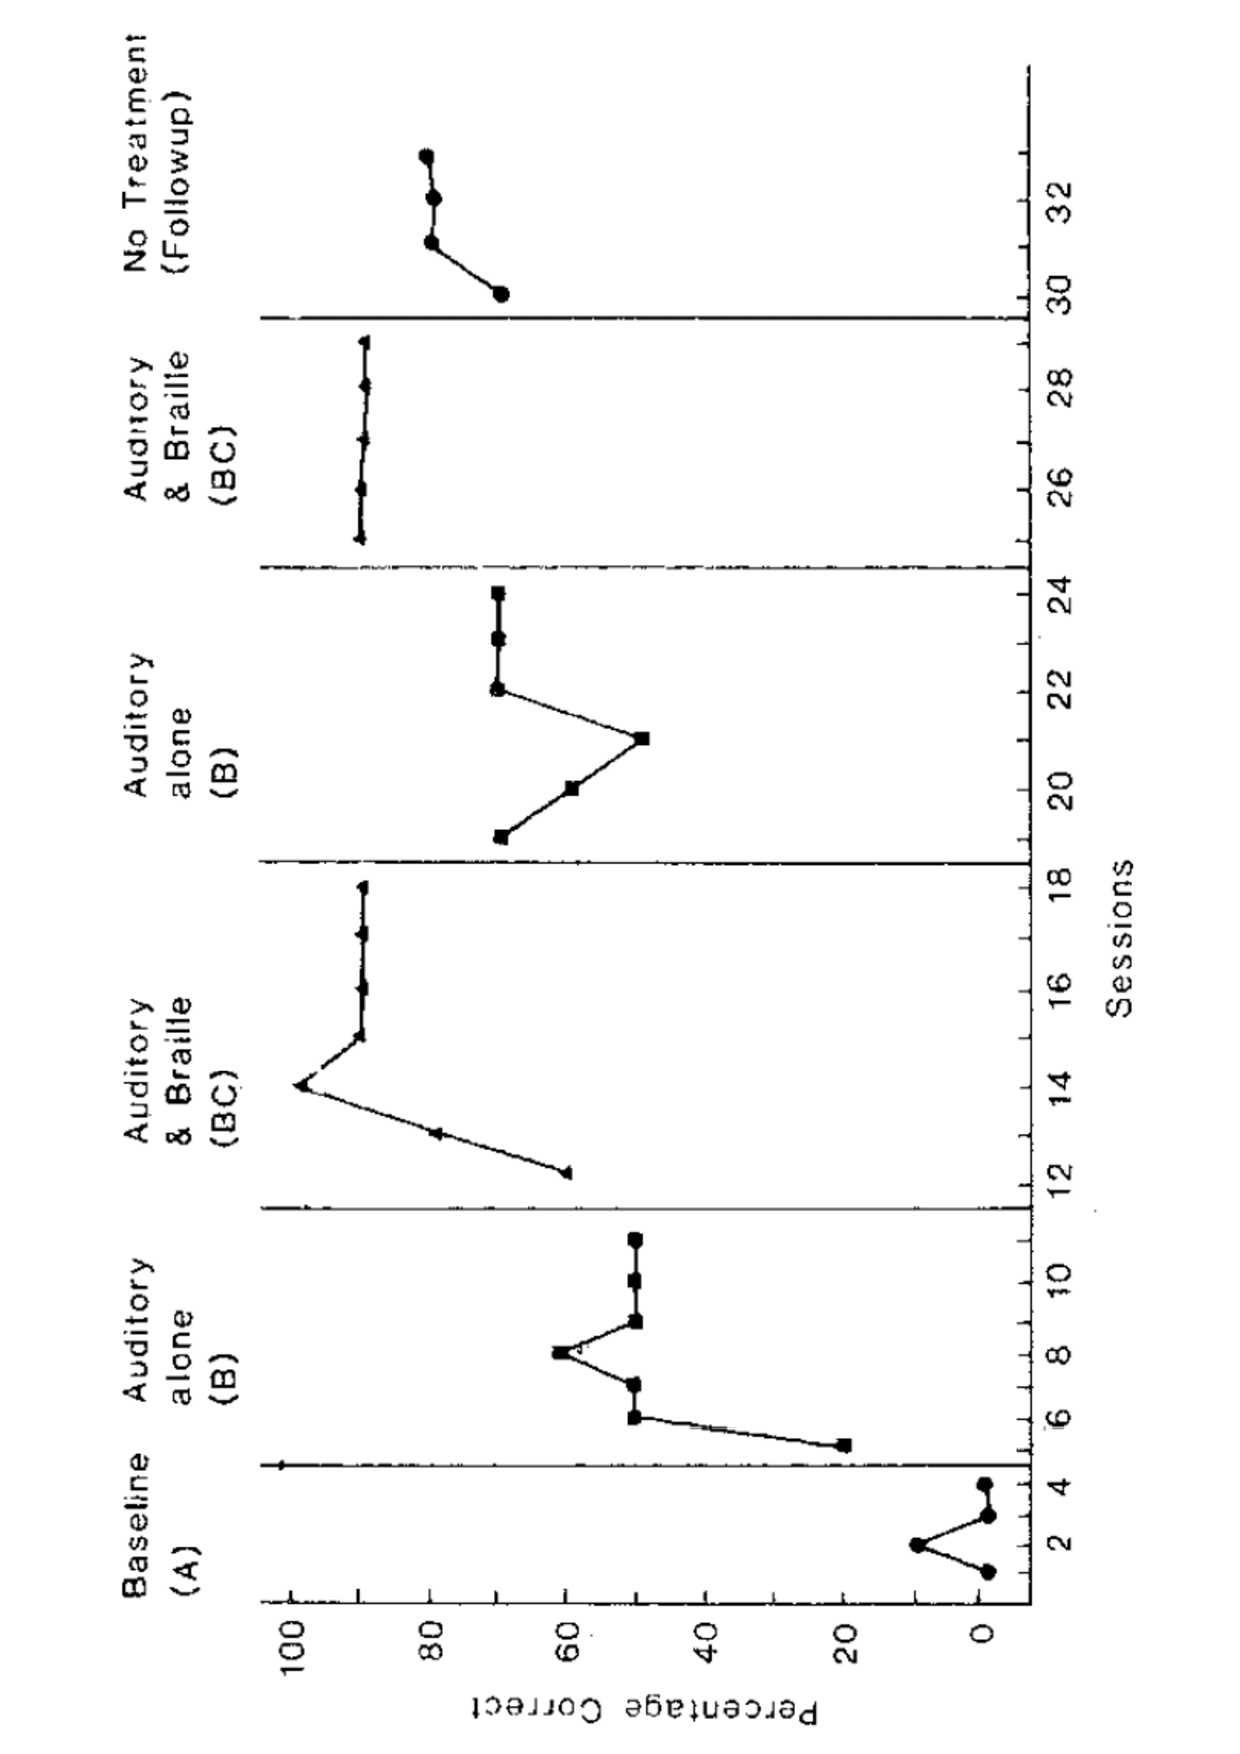
\includegraphics[angle=270, width=9cm]{images/kearns1986_Fig3.pdf}
	\end{center}
\end{frame}

\section{Data analysis, reporting, appraisal}

% 
\begin{frame}{Data analysis and interpretation}
	\begin{itemize}
	\item Graph baseline and intervention probe results and visually interpret it (covered in last session)
	\item Calculate an effect size measure\footnote{\tiny{See \citet{Rakap2015} for further information and sample calculations.}}
		\begin{enumerate}
		\item Percentage of non-overlapping data (PND)
		\item Improvement rate differences (IRD)
		\item Percentage of data exceeding a median trend (PEM-T)
		\item Tau for non-overlap with baseline trend control (Tau-\emph{U})
		\end{enumerate}
	\end{itemize}
\end{frame}

%
\begin{frame}{Example from \citet{Rakap2015}}
	\begin{center}
	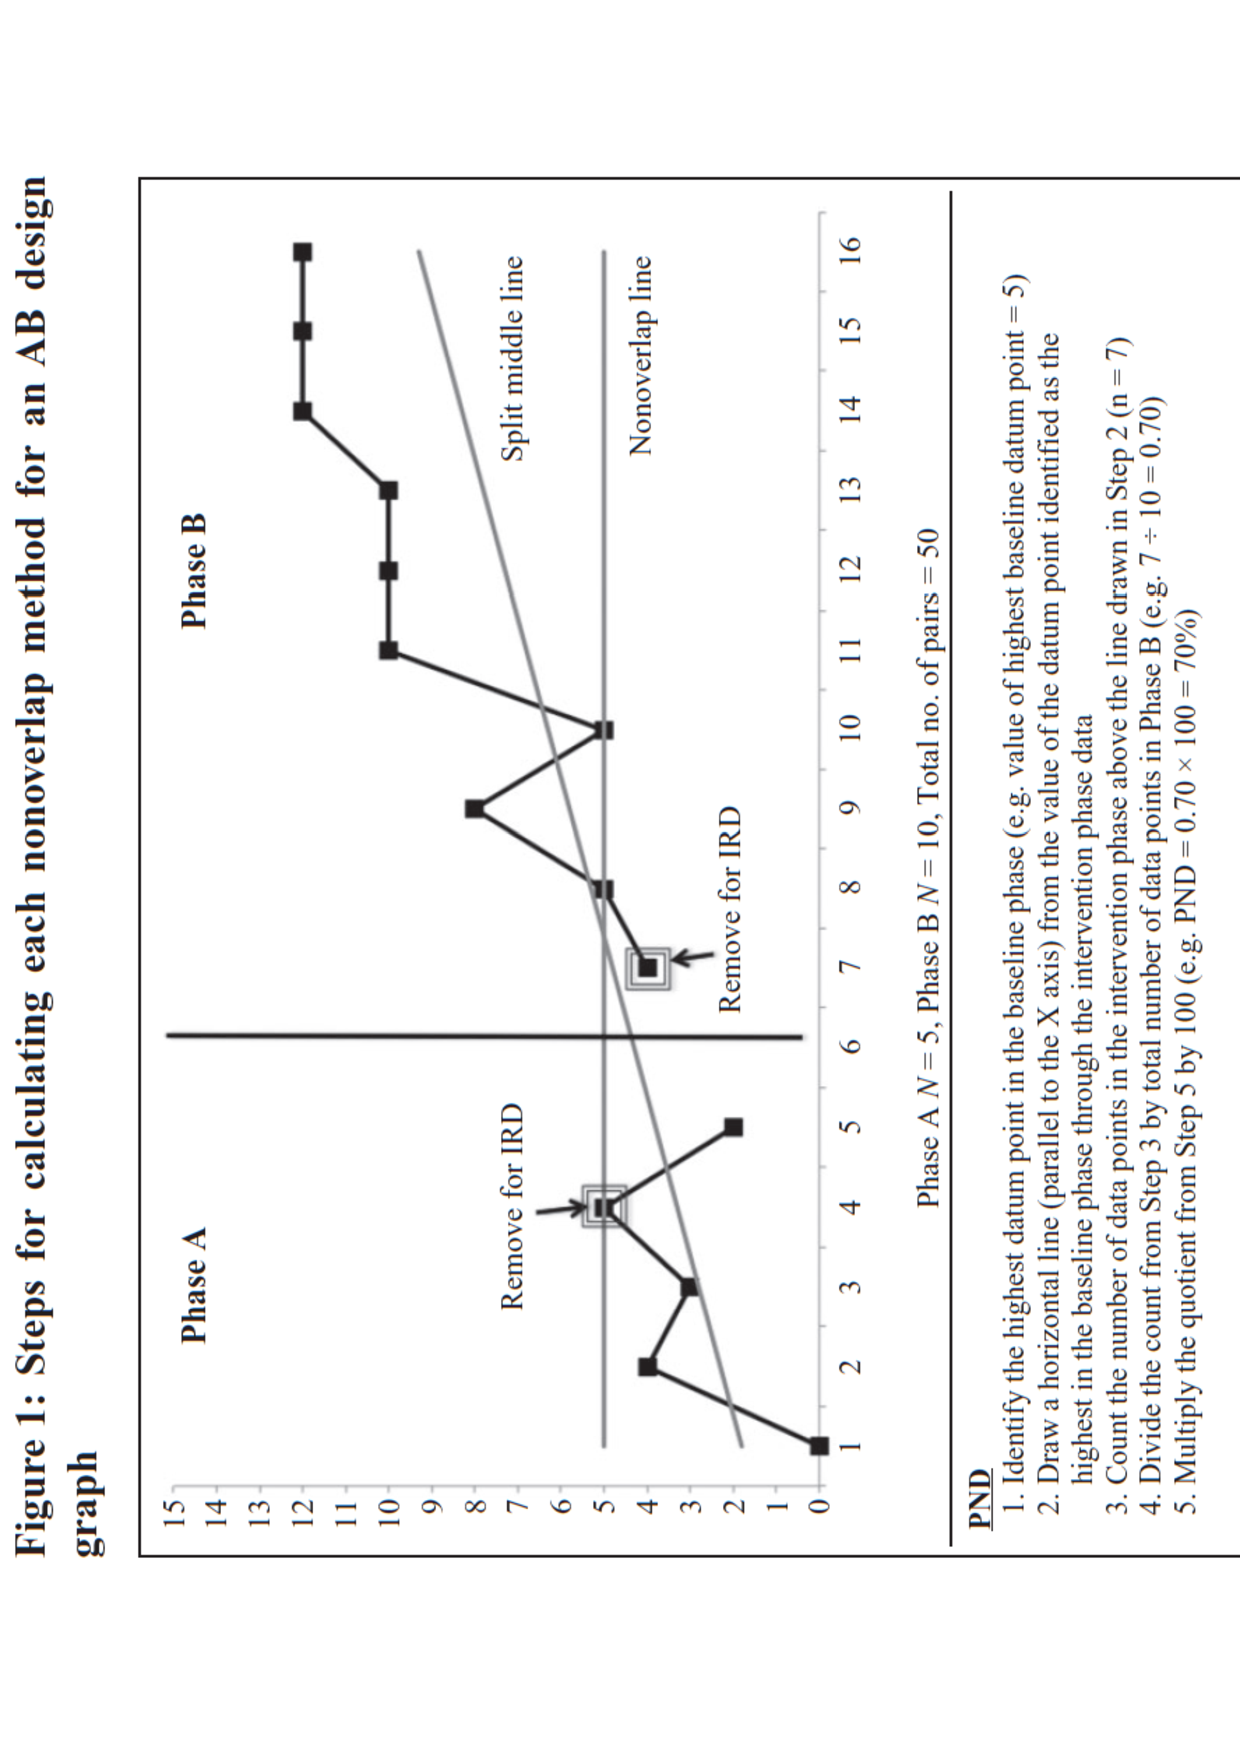
\includegraphics[angle=270, width=10cm]{images/Rakap_Fig1.pdf}
	\end{center}
\end{frame}

%
\begin{frame}{Example from \citet{Rakap2015}}
	\begin{center}
	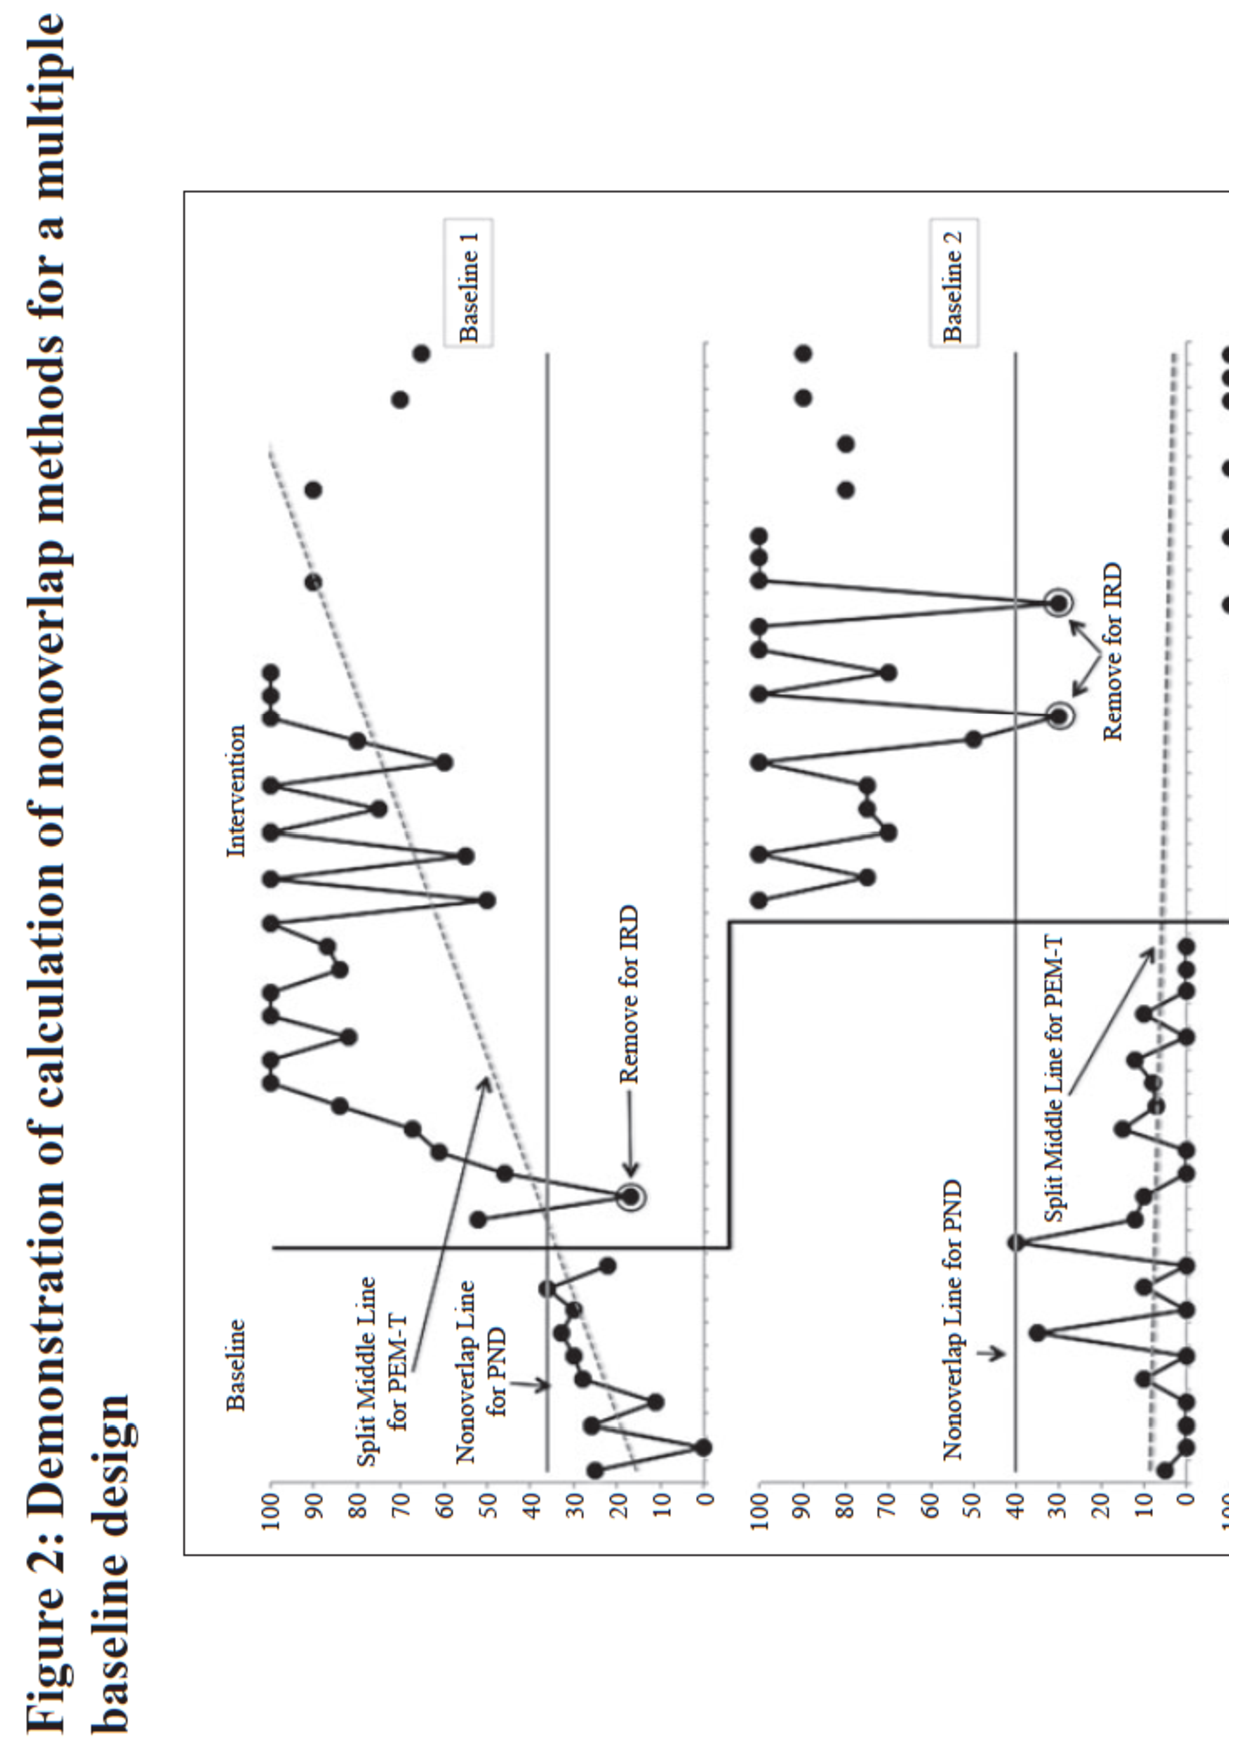
\includegraphics[angle=270, width=10cm]{images/Rakap_Fig2.pdf}
	\end{center}
\end{frame}

% 
\begin{frame}{SSD evidence hierarchy\footnote{\tiny{\citet[p.100]{Logan2008}}}}
	\begin{center}
	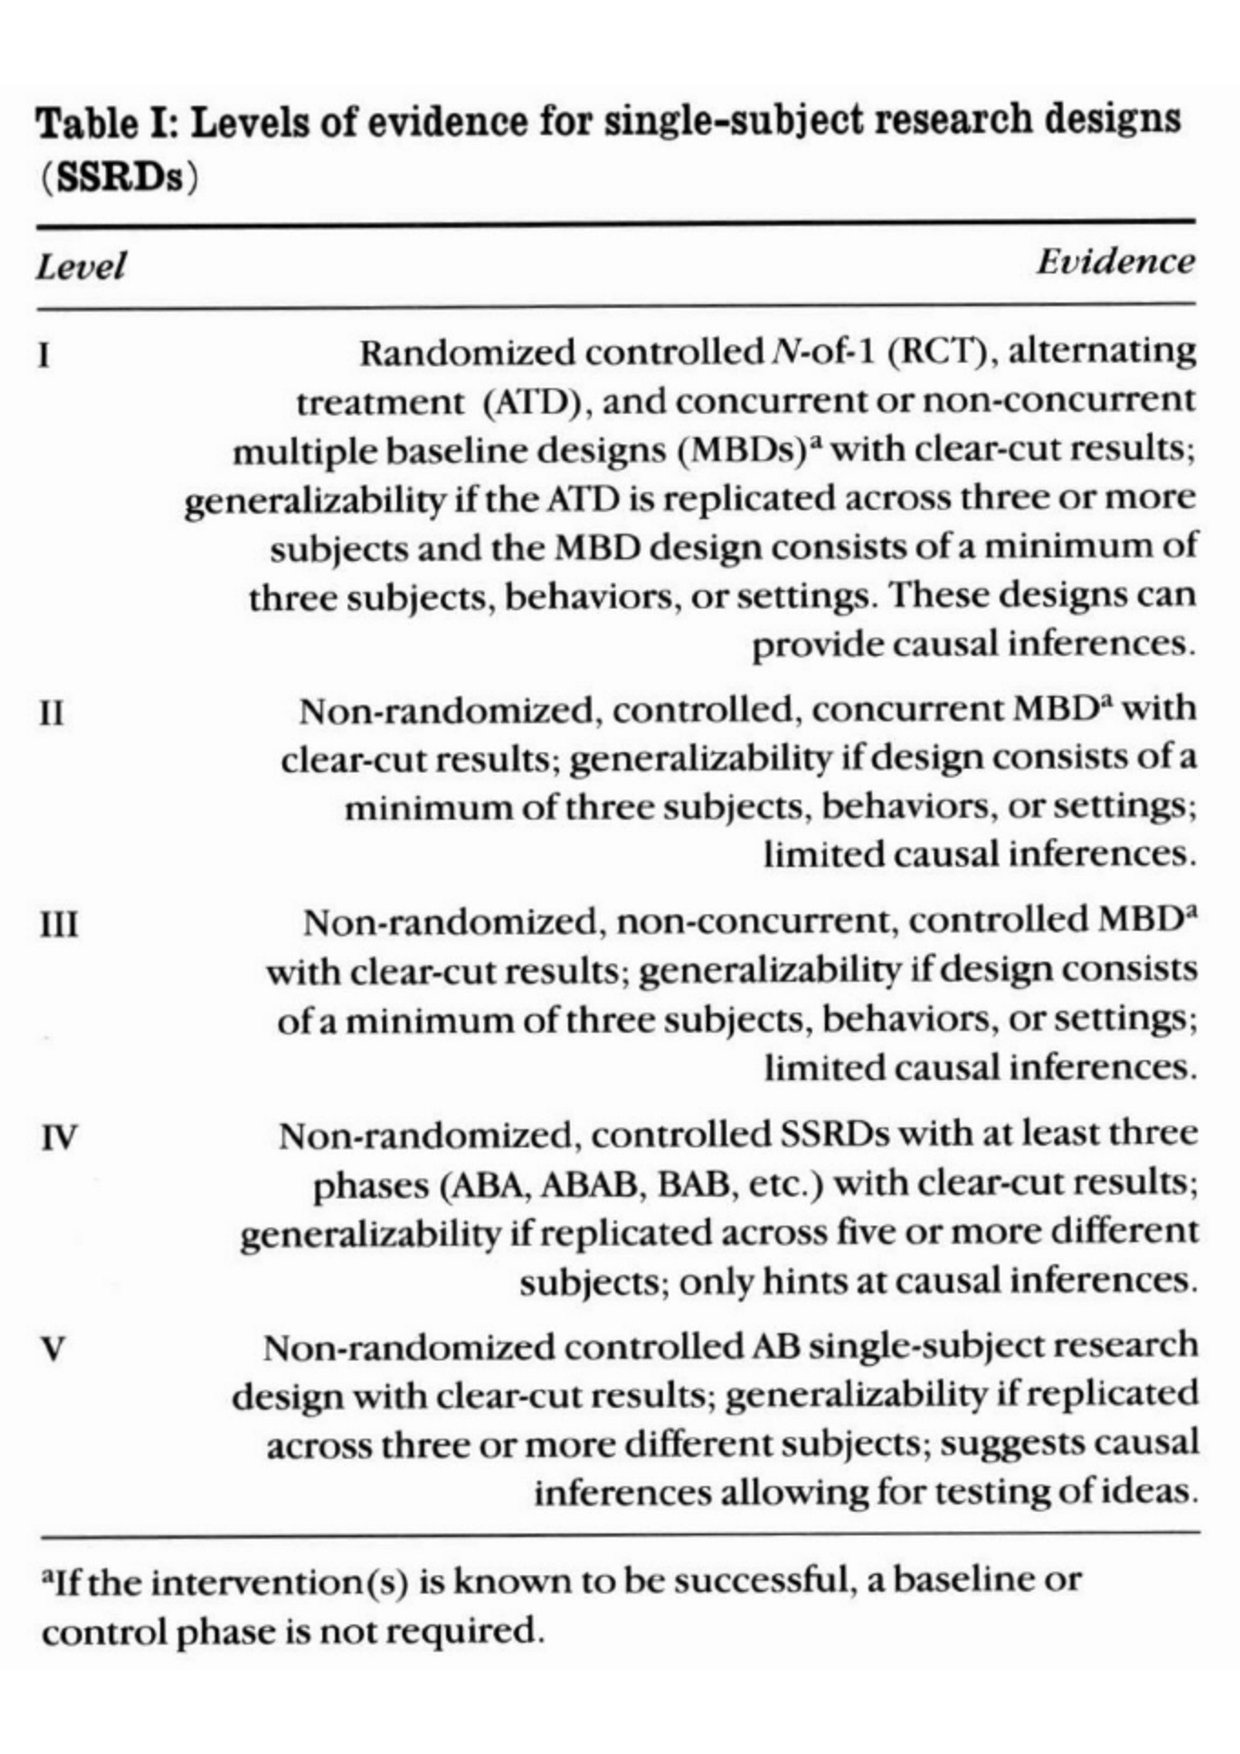
\includegraphics[width=5cm]{images/Logan2008_table1.pdf}
	\end{center}
\end{frame}

% 
\begin{frame}{Reporting standards for SSDs}
	\begin{itemize}
	\item To promote transparent and complete reporting of SSDs
	\item The \emph{Single-Case Reporting Guideline in BEhavioural Interventions} (SCRIBE) 2016 checklist \citep{Tate2016a}
		\begin{itemize}
		\item For authors of SSDs
		\item 26-item checklist + flow diagram
		\end {itemize}
	\item The \emph{Journal Article Reporting Standards for Quantitative Research in Psychology} (JARS) \citep{Appelbaum2018}
		\begin{itemize}
		\item Now includes section on reporting SSDs (see Table 3)
		\end{itemize}
	\end {itemize}
\end{frame}

% 
\begin{frame}{Options for critically appraising SSDs}
	\begin{itemize}
	\item Single Case Experimental Design Scale (SCED) Scale \citep{Tate2008}
	\item Logan et al.'s 14-item checklist \citep[p. 102]{Logan2008}	
	\item CATE \citep{Dollaghan2007a}
	\end{itemize}
\end{frame}

\section{Group Discussion}

% 
\begin{frame}{Group discussion}
	\begin{itemize}
	\item Break up into your assigned groups.
	\item Use SCED \citep[pp. 400-1]{Tate2008} to critically appraise the study.
	\item Document where you found information in the research article addressing each point.
	\end{itemize}
\end{frame}

\begin{frame}[allowframebreaks] %[shrink=15]
	\frametitle{References}
	\bibliographystyle{apacite}
	\small\bibliography{/Users/thomasklee/Documents/Bibtex/library}
\end{frame}

\end{document}